\documentclass[12pt, letterpaper]{article}
\usepackage[english]{babel}
\usepackage{amsmath}
\usepackage{unicode-math}
\usepackage[margin=0.7in]{geometry}
\usepackage{graphicx}
%\usepackage{mathrsfs}
\usepackage{fontspec}
\setmainfont{Calibri}
% must be compiled with XeLaTeX, not pdfLaTeX

  %%%%%%%%%%%%
  % PREAMBLE %
  %%%%%%%%%%%%
\begin{document}
\selectlanguage{english}

\section*{Postrefinement: The model {\tt rs}. }
  \par This is intended to be the simplest possible model for the reciprocal lattice point (RLP), 
  describing the RLP as a sphere of radius ${r_s}$, which is globally constant over the whole dataset
  consisting of an ensemble of crystal lattices (or frames).  
\subsection*{1 The size of the RLP model}

  \par The constant value of ${r_s}$ is computed as follows.
  From model refinement and integration, each crystal has associated with it a list of Miller indices 
  $\mathbf{h_i}$ and a reciprocal space orientation matrix $\mathbf{A}$ 
  defined by Rossmann $\textit{et\ al.}$ (1979),
    \begin{equation}
    \mathbf{A} = 
    \left(
    \begin{array}{c c c}
      a_{x}^{*}   &  b_{x}^{*}   & c_{x}^{*}  \\
      a_{y}^{*}   &  b_{y}^{*}   & c_{y}^{*}  \\
      a_{z}^{*}   &  b_{z}^{*}   & c_{z}^{*}  \\
    \end{array}
    \right)
    \text{.}
    \label{eqn:RossmannA}
  \end{equation}
  The reciprocal space coordinates of RLP $i$ are computed with 
    \begin{equation}
    \mathbf{q} = \mathbf{A}\mathbf{h}
    \text{,}
    \label{eqn:Ah}
  \end{equation}
  leading to a reciprocal position Q, with a small distance offset
   ${r_h}$ away from the Ewald sphere that represents the perfect diffracting condition.  
  The fact that $|{r_h}|$ is non-zreo is indicative that
  Bragg observations from still shots represent partial reflections.  Note that array index $i$ denoting
  a specific Miller index is dropped on occasion for clarity.  The geometry is explained in Fig. 1. 
  
  \begin{figure}[htb]
  \begin{center}
  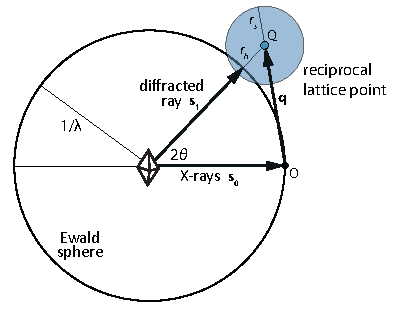
\includegraphics[scale=1.5]{Figure_1.pdf}
  \label{fig:1}
  \end{center}
  \begin{center}
  {Fig. 1. Ewald sphere construction.}
  \end{center}
  \end{figure}

  The quantity $|{r_h}|$ is given by 
    \begin{equation}
    {r_h} = ||\mathbf{q}+\mathbf{s_0}||-||\mathbf{s_1}|| = ||\mathbf{q}+\mathbf{s_0}||-\dfrac{1}{ \lambda}
    \text{,}
    \label{eqn:Rh}
  \end{equation}

  where ${s_0}$ and ${s_1}$ are respectively the beam vector and the diffracted ray vector,
  each of length $1/\lambda$.  For the model {\tt rs}, the constant value of ${r_s}$ is taken 
  as the root mean-squared value of
  ${r_h}$ over all Bragg spots integrated from a given crystal.  It therefore depends on whatever
  algorithm has been used to predict spots, regardless of whether there is measurable signal
  in the spots.  
  \subsection*{2 The geometry of the RLP model}

  \par The intention is to create a model of the RLP similar to a hard sphere, so that if any portion 
  of the sphere touches the Ewald sphere there is signal expected, otherwise none.  However, this 
  is a discontinuous model (in terms of the spot partiality expressed as a function of ${r_h}$ and
  therefore not easily amenable to parameter fitting.  Therefore we relax the requirement for a hard
  sphere and adopt a radial profile somewhat smoother.  For the Uervirojnangkoorn (2015) paper
  we used a profile based on a Lorentzian function.  The derivation is as follows.  
  
\par A suggestion from James Holton defines the Bragg spot partiality as
  
  \begin{equation}
    p = \frac{\text{Area of intersection between the Ewald sphere and } F_{hkl}}
             {\text{Area of intersection between the Ewald sphere and } F_{000}}
    \text{.}
    \label{eqn:part}
  \end{equation}
  
The "areas of intersection" in question are really spherical caps that represent the Ewald 
sphere's intersection with the reciprocal space ball of radius $r_s$.  However, we're not going to 
insist on such detail; instead we will simply take a circular area of radius $r_p$ such that we
have the right triangle

  \begin{equation}
    {r}_p^2 = {r}_s^2 - {r}_h^2
    \text{,}
    \label{eqn:pyth}
  \end{equation}

and then the approximate expression for partiality becomes (model A),

  \begin{equation}
    p_A = \frac{\pi r_p^2}{\pi r_s^2} = 1 - \frac{r_h^2}{r_s^2} \text{ for }|r_h|<r_s, 0 \text{ otherwise}
    \text{.}
    \label{eqn:fexprr}
  \end{equation}

Partiality as a function of $r_h$ is a simple inverted parabola with $p_A=1$ at $r_h=0$ and 
roots at $\pm r_s$ (Fig. 2).  Outside of this domain the partiality is 0. 

  \begin{figure}[htb!]
  \begin{center}
  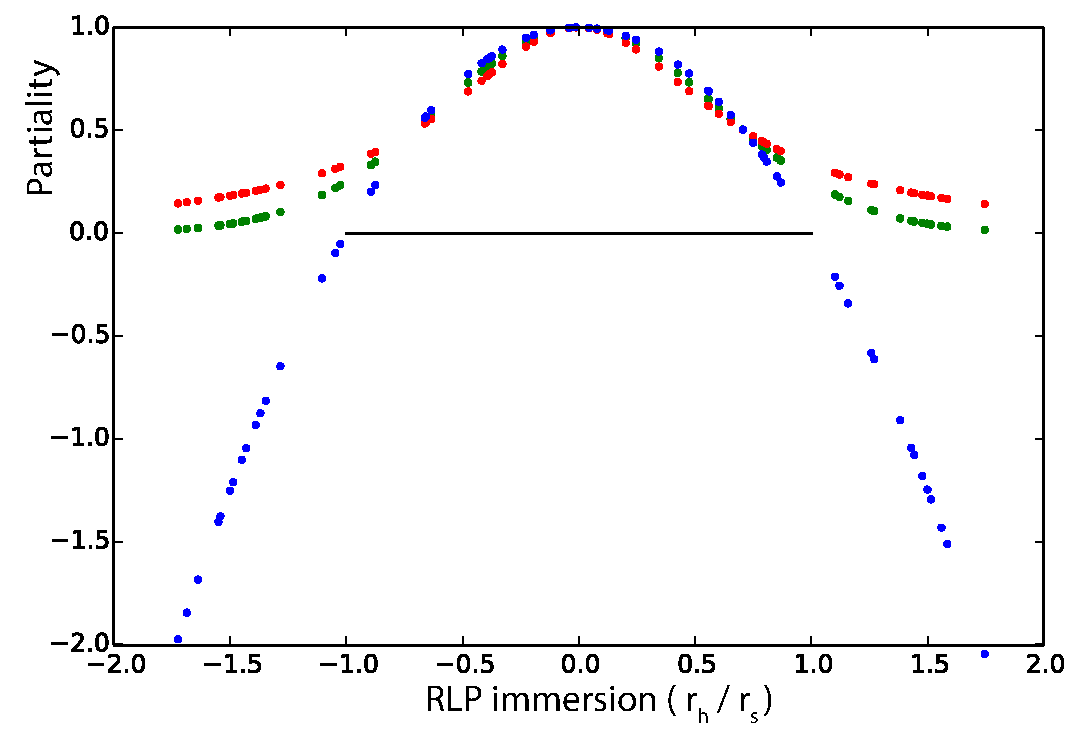
\includegraphics[scale=0.65]{Figure_2.pdf}
  %\includesvg{Figure_2}
  \label{fig:2}
  \end{center}
  \begin{center}
  {Fig. 2. Two partiality models:  a simple hard-sphere model ($p_A$, blue), and a soft-sphere Lorentzian
  function ($p_B$, red).}
  \end{center}
  \end{figure}

However, having a 
mathematically discontinuous
expression ($p_A$) will leave us at a disadvantage for postrefinement.  The postrefinement strategy  
will be to express the lack of closure $r_h$ in terms of model parameters such as the unit cell
dimensions and crystal orientation.  Then optimize a target function $f$ expressed in 
terms of the partiality $p$, attempting to find parameter values to minimize $f$.  It is 
crucial in this procedure to have an expression for partiality that is smooth and differentiable. 

We will therefore have to modify our simple model of the Bragg spot as a reciprocal space ball.  
One functional form that might have the desired properties is the Lorentzian function
  \begin{equation}
    L = \frac{1}{\pi}\frac{\frac{1}{2}\Gamma}{x^2 + (\frac{1}{2}\Gamma)^2}
    \text{,}
    \label{eqn:loren}
  \end{equation}
where $\Gamma$ is the full-width at half maximum (FWHM).  

Let's tinker with this expression so it conforms to expectation...first multiply by 
a scaling constant to get $L'(0)=1$:
  \begin{equation}
    L^{\prime} = \frac{\pi \Gamma}{2}L
    \text{,}
    \label{eqn:lorenA}
  \end{equation}

and finally setting the FWHM to the FWHM value obtained from eqn \eqref{eqn:fexprr},
  \begin{equation}
    \Gamma = \frac{2r_s}{\sqrt{2}}
    \text{,}
    \label{eqn:fwhm}
  \end{equation}
so we get a new partiality expression (model B):

  \begin{equation}
    p_B = \frac{r_s^2}{2r_h^2 + r_s^2}
    \text{.}
    \label{eqn:pb}
  \end{equation}

Finally, for postrefinement we'll need the partial derivative of $p_B$ with respect to $r_h$ (use the 
quotient rule):
  \begin{equation}
    \frac{\partial{p_B}}{\partial{r_h}} = \frac{-4r_s^2r_h}{(2r_h^2 + r_s^2)^2}
    \text{.}
    \label{eqn:deriv}
  \end{equation}


  \subsection*{3 Model parameters and target function}
  \par The goal of this work is to refine the parameters of the partiality model so that the 
  observed intensities, corrected to their full spot equivalents, offer the best agreement over
  repeated measurements of the same asymmetric-unit Miller index.  In practice,
  the parameters representing each crystal lattice are refined 
  against a set of reference intensities $I_{\mathrm{ref}}$.  
  Program {\it prime} uses simple scaling to create an initial reference, after which repeated 
  cycles of postrefinement are performed, with the reference being created from the corrected, 
  merged intensities from the previous cycle.  In {\it cxi.merge} the reference is an isomorphous
  atomic structure, from which intensities $I_{\mathrm{ref}}$ are calculated, and only one 
  cycle is performed.  The polarization-corrected measurements are denoted $I_{\mathrm{obs}}$.
  The parameters refined for each crystal lattice are:
  
  \par $G$: the scale factor.
  \par $B$: the Wilson $B$-factor.
  \par $\theta_{x}$: incremental crystal rotation angle on $x$-axis ($\perp$ to beam).
  \par $\theta_{y}$: incremental crystal rotation angle on $y$-axis ($\perp$ to beam).
  \par The least-squares target function used to achieve best agreement between model and 
  observation is 
  
  
  \begin{equation}
 \mathscr{F} =  \sum_{i} \limits
    ( G  \exp(\dfrac{-8B\sin^2\theta}{\lambda^2}) p_B I_{\mathrm{ref}} - I_{\mathrm{obs}})^{2}
\end{equation}
where $\theta$ is the Bragg diffraction angle defined in Fig. 1, and $\lambda$ the wavelength, both 
treated as constants, and the sum is over all measurements integrated from a single crystal lattice. 

  \subsection*{4 Necessary derivatives for parameter refinement}

  \par Given the least-squares form, derivatives of the target functional with respect to 
  parameter $\mathscr{P}$ are in general
  
    \begin{equation}
    \frac{\partial\mathscr{F}}{\partial\mathscr{P}} = 2\sum_{i} \limits
    \mathscr{R}_i\dfrac{\partial\mathscr{R}_i}{\partial\mathscr{P}}
    \text{,}
    \label{eqn:genFP}
  \end{equation}
where the residual comparison on each observation is 

  \begin{equation}
 \mathscr{R}_i =  
    G  \exp(\dfrac{-8B\sin^2\theta}{\lambda^2}) p_B I_{\mathrm{ref}} - I_{\mathrm{obs}}
    \text{.}
    \end{equation}
The derivatives in the Jacobian matrix, required for parameter optimization, are more-or-less
straightforward:

    \begin{equation}
    \frac{\partial\mathscr{R}_i}{\partial G} = 
    \exp(\dfrac{-8B\sin^2\theta}{\lambda^2}) p_B I_{\mathrm{ref}}
    \text{,}
    \label{eqn:dG}
  \end{equation}

     \begin{equation}
    \frac{\partial\mathscr{R}_i}{\partial B} = 
    G  \exp(\dfrac{-8B\sin^2\theta}{\lambda^2}) p_B I_{\mathrm{ref}}
    \left( \dfrac{-8\sin^2\theta}{\lambda^2}\right)
    \text{.}
    \label{eqn:dB}
  \end{equation}

  \par The derivatives with respect to $\theta_{x}$ and $\theta_{y}$ require more work.  All of the
  dependence on crystal orientation comes through the expression for partiality:
  
      \begin{equation}
    \frac{\partial\mathscr{R}_i}{\partial \theta_{x\mathrm{|}y}} = 
  \frac{\partial\mathscr{R}_i}{\partial p_B}
   \frac{\partial p_B} {\partial \theta_{x\mathrm{|}y}}
    \text{,}
    \label{eqn:dthxy}
  \end{equation}

with

      \begin{equation} 
  \frac{\partial\mathscr{R}_i}{\partial p_B} =
  G  \exp(\dfrac{-8B\sin^2\theta}{\lambda^2}) I_{\mathrm{ref}}
    \text{.}
    \label{eqn:P_terms}
  \end{equation}

As for the variation of the partiality model $p_B$ defined in \eqref{eqn:pb}, the {\tt rs}
model assumes that the sphere radius $r_s$ is fixed, thus the only remaining variable is the
distance  $r_h$ between RLP and Ewald sphere:

   \begin{equation}
   \frac{\partial p_B} {\partial \theta_{x\mathrm{|}y}} = 
  \frac{\partial p_B}{\partial r_h}
   \frac{\partial r_h} {\partial \theta_{x\mathrm{|}y}}
    \text{.}
    \label{eqn:dpb2}
  \end{equation}


  \par An expression for $\dfrac{\partial p_B}{\partial r_h}$ has already been 
  given in \eqref{eqn:deriv}, so it now
  remains to investigate the derivative $\dfrac{\partial r_h} {\partial \theta_{x\mathrm{|}y}}$,
  based on the definition of $r_h$ given in \eqref{eqn:Rh}.

Introduce the vector $\mathbf{S}$:
   \begin{equation}
   \mathbf{S} = \mathbf{q}+\mathbf{s_0}
    \text{,}
    \label{eqn:SS}
  \end{equation}

   \begin{equation}
 {r_h} = ||\mathbf{S}||-\dfrac{1}{ \lambda}
     \text{,}
    \label{eqn:sss}
  \end{equation}
  
    \begin{equation}
   \dfrac{\partial r_h} {\partial \theta_{x\mathrm{|}y}} = 
   \dfrac
   {\mathbf{S}\cdot{
   \dfrac{\partial \mathbf{S}} {\partial \theta_{x\mathrm{|}y}}
   }}
   {||\mathbf{S}||}
    \text{,}
    \label{eqn:rhth}
  \end{equation}

    \begin{equation}
   \dfrac{\partial \mathbf{S}} {\partial \theta_{x\mathrm{|}y}} = 
  {
   \dfrac{\partial \mathbf{q}} {\partial \theta_{x\mathrm{|}y}}
   }
    \text{.}
    \label{eqn:derivsq}
  \end{equation}

Finally we investigate the derivative of the RLP position $\mathbf{q}$ with respect to the crystal 
rotations.  The effective orientation matrix $\mathbf{A}$ may be expressed as the 
reference orientation matrix $\mathbf{A}_\mathrm{ref}$ determined during crystal refinement and 
integration, composed with additional rotational operators $\mathbb{R}_x$ and 
$\mathbb{R}_y$ determined by the postrefined angles $\theta_{x}$ and 
$\theta_{y}$:

    \begin{equation}
   \mathbf{A} = 
\mathbb{R}_y( \mathbb{R}_x ( \mathbf{A}_\mathrm{ref} )  )
    \text{.}
    \label{eqn:compoase}
  \end{equation}

The derivatives of $\mathbf{q}$ work out as follows:

  \begin{equation}
   \dfrac{\partial \mathbf{q}} {\partial \theta_{x}} = 
  \mathbb{R}_y \dfrac{\partial\mathbb{R}_x}{\partial \theta_{x}}  \mathbf{A}_\mathrm{ref} \mathbf{h}
    \text{,}
    \label{eqn:qthx}
  \end{equation}
  \begin{equation}
   \dfrac{\partial \mathbf{q}} {\partial \theta_{y}} = 
  \dfrac{\partial\mathbb{R}_y}{\partial \theta_{y}} \mathbb{R}_x \mathbf{A}_\mathrm{ref} \mathbf{h}
    \text{.}
    \label{eqn:qthy}
  \end{equation}

The derivatives of the rotation operator are already encoded in the cctbx library ({\tt scitbx/matrix/\_\_init\_\_.py}).  Formulae for the rotation operator and its derivative with 
respect to angle $\theta$ are given in the LaTeX documentation included in that directory.
%%%%%%%%%%%%%%%%%%%%%


\end{document}
